% biography section
% 
% If you have an EPS/PDF photo (graphicx package needed) extra braces are
% needed around the contents of the optional argument to biography to prevent
% the LaTeX parser from getting confused when it sees the complicated
% \includegraphics command within an optional argument. (You could create
% your own custom macro containing the \includegraphics command to make things
% simpler here.)
%\begin{IEEEbiography}[{\includegraphics[width=1in,height=1.25in,clip,keepaspectratio]{mshell}}]{Michael Shell}
% or if you just want to reserve a space for a photo:

%\begin{IEEEbiography}{Michael Shell}
%Biography text here.
%\end{IEEEbiography}

% if you will not have a photo at all:
%\begin{IEEEbiographynophoto}{John Doe}
%Biography text here.
%\end{IEEEbiographynophoto}

% insert where needed to balance the two columns on the last page with
% biographies
\newpage

%\begin{IEEEbiographynophoto}{Jane Doe}
%Biography text here.
%\end{IEEEbiographynophoto}

% You can push biographies down or up by placing
% a \vfill before or after them. The appropriate
% use of \vfill depends on what kind of text is
% on the last page and whether or not the columns
% are being equalized.

\begin{IEEEbiography}
[{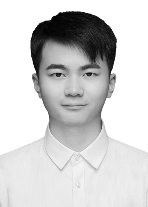
\includegraphics[width=1in,height=1.25in,clip,keepaspectratio]{./figs/szx.pdf}}]
{Zhuoxue Song} received the B.S. degree in computer science and technology from Hangzhou Dianzi University, in 2021. 
He is currently working toward the M.S. degree in the security of cyberspace at Zhejiang University. 
His main research interests include encrypted traffic classification and intrusion detection.
\end{IEEEbiography}

\begin{IEEEbiography}
[{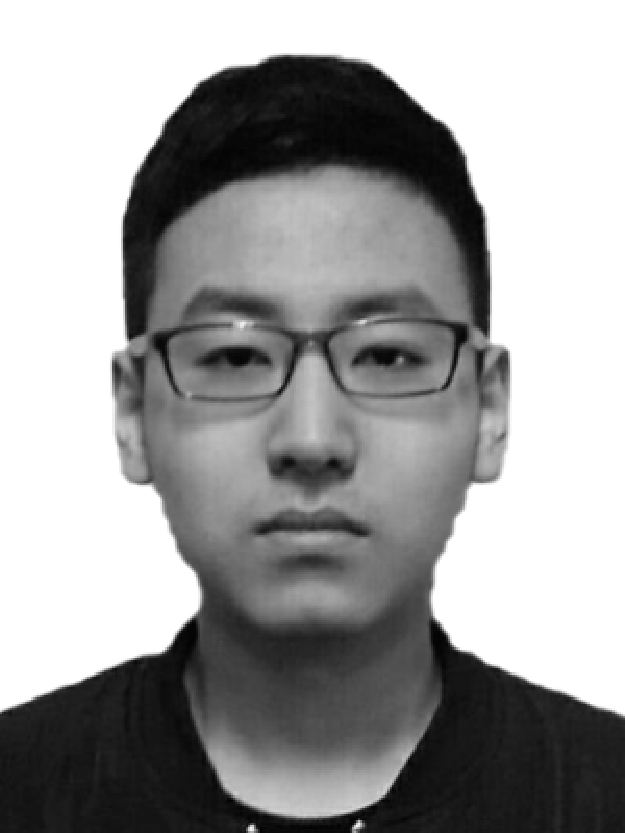
\includegraphics[width=1in,height=1.25in,clip,keepaspectratio]{./figs/zzm.pdf}}]
{Ziming Zhao} received the B.S. degree in computer science and technology from Shijiazhuang Tiedao University, in 2019.
He is currently working toward the Ph.D. degree in the security of cyberspace at Zhejiang University. 
His main research interests include network security and intrusion detection.
\end{IEEEbiography}

\begin{IEEEbiography}
[{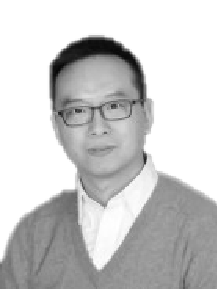
\includegraphics[width=1in,height=1.25in,clip,keepaspectratio]{./figs/zf.pdf}}]
{Fan Zhang} (Member,~IEEE) received the Ph.D. degree from the Department of Computer Science and Engineering, University of Connecticut, Mansfield, CT, USA, in 2011.
He is currently a Full Professor with the College of Computer Science and Technology, Zhejiang University, Hangzhou, China, and also with the Alibaba–Zhejiang University Joint Institute of Frontier Technologies, Hangzhou. 
His research interests include system security, hardware security, network security, and cryptography.
\end{IEEEbiography}

\begin{IEEEbiography}
[{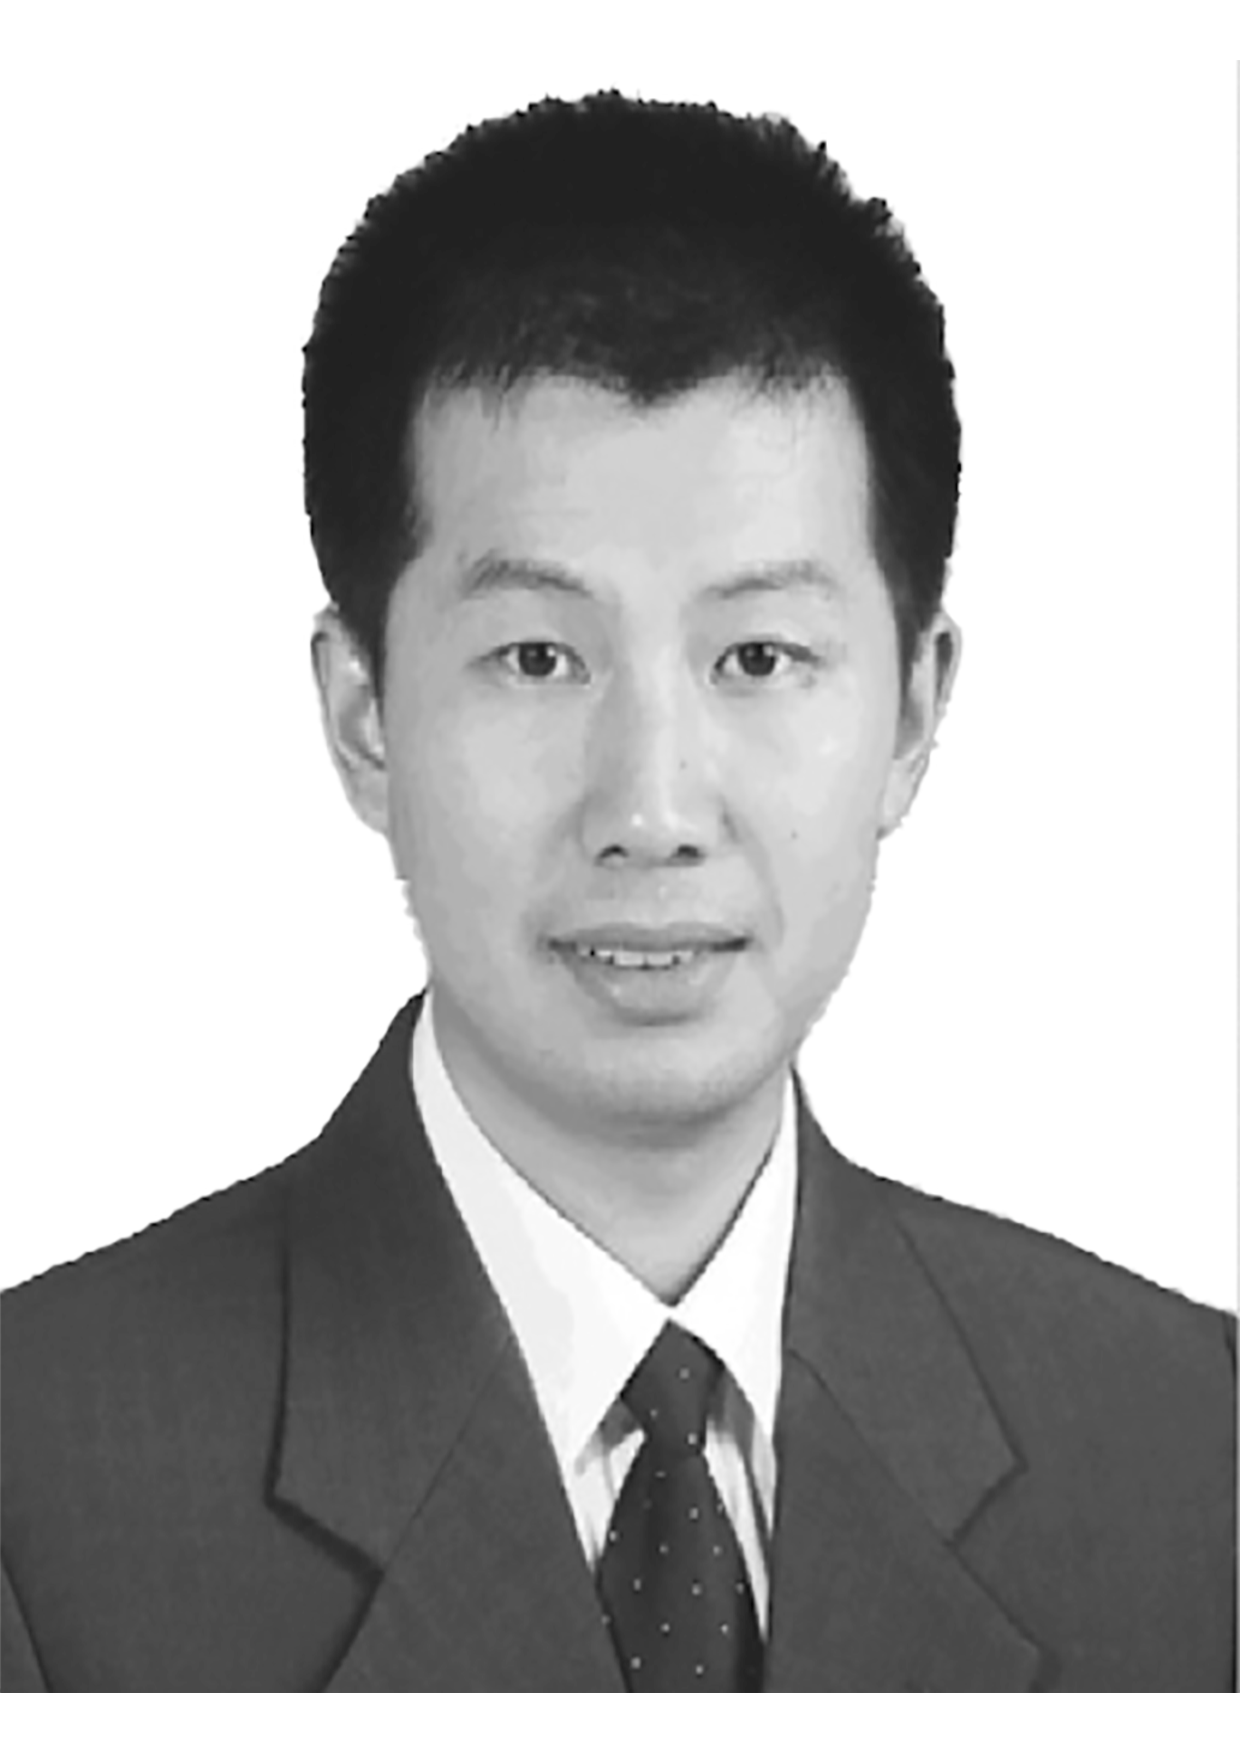
\includegraphics[width=1in,height=1.25in,clip,keepaspectratio]{./figs/xg.pdf}}]
{Gang Xiong} is currently a Full Professor and Ph.D. Supervisor with the Institute of Information Engineering, Chinese Academy of Sciences, China. He has authored more than 60 papers in refereed journals and conference proceedings. His research interests include network and information security. He is a member of the 3rd Communication Security Technical Committee of China Institute of Communications.
\end{IEEEbiography}
\vfill
\newpage
\begin{IEEEbiography}
[{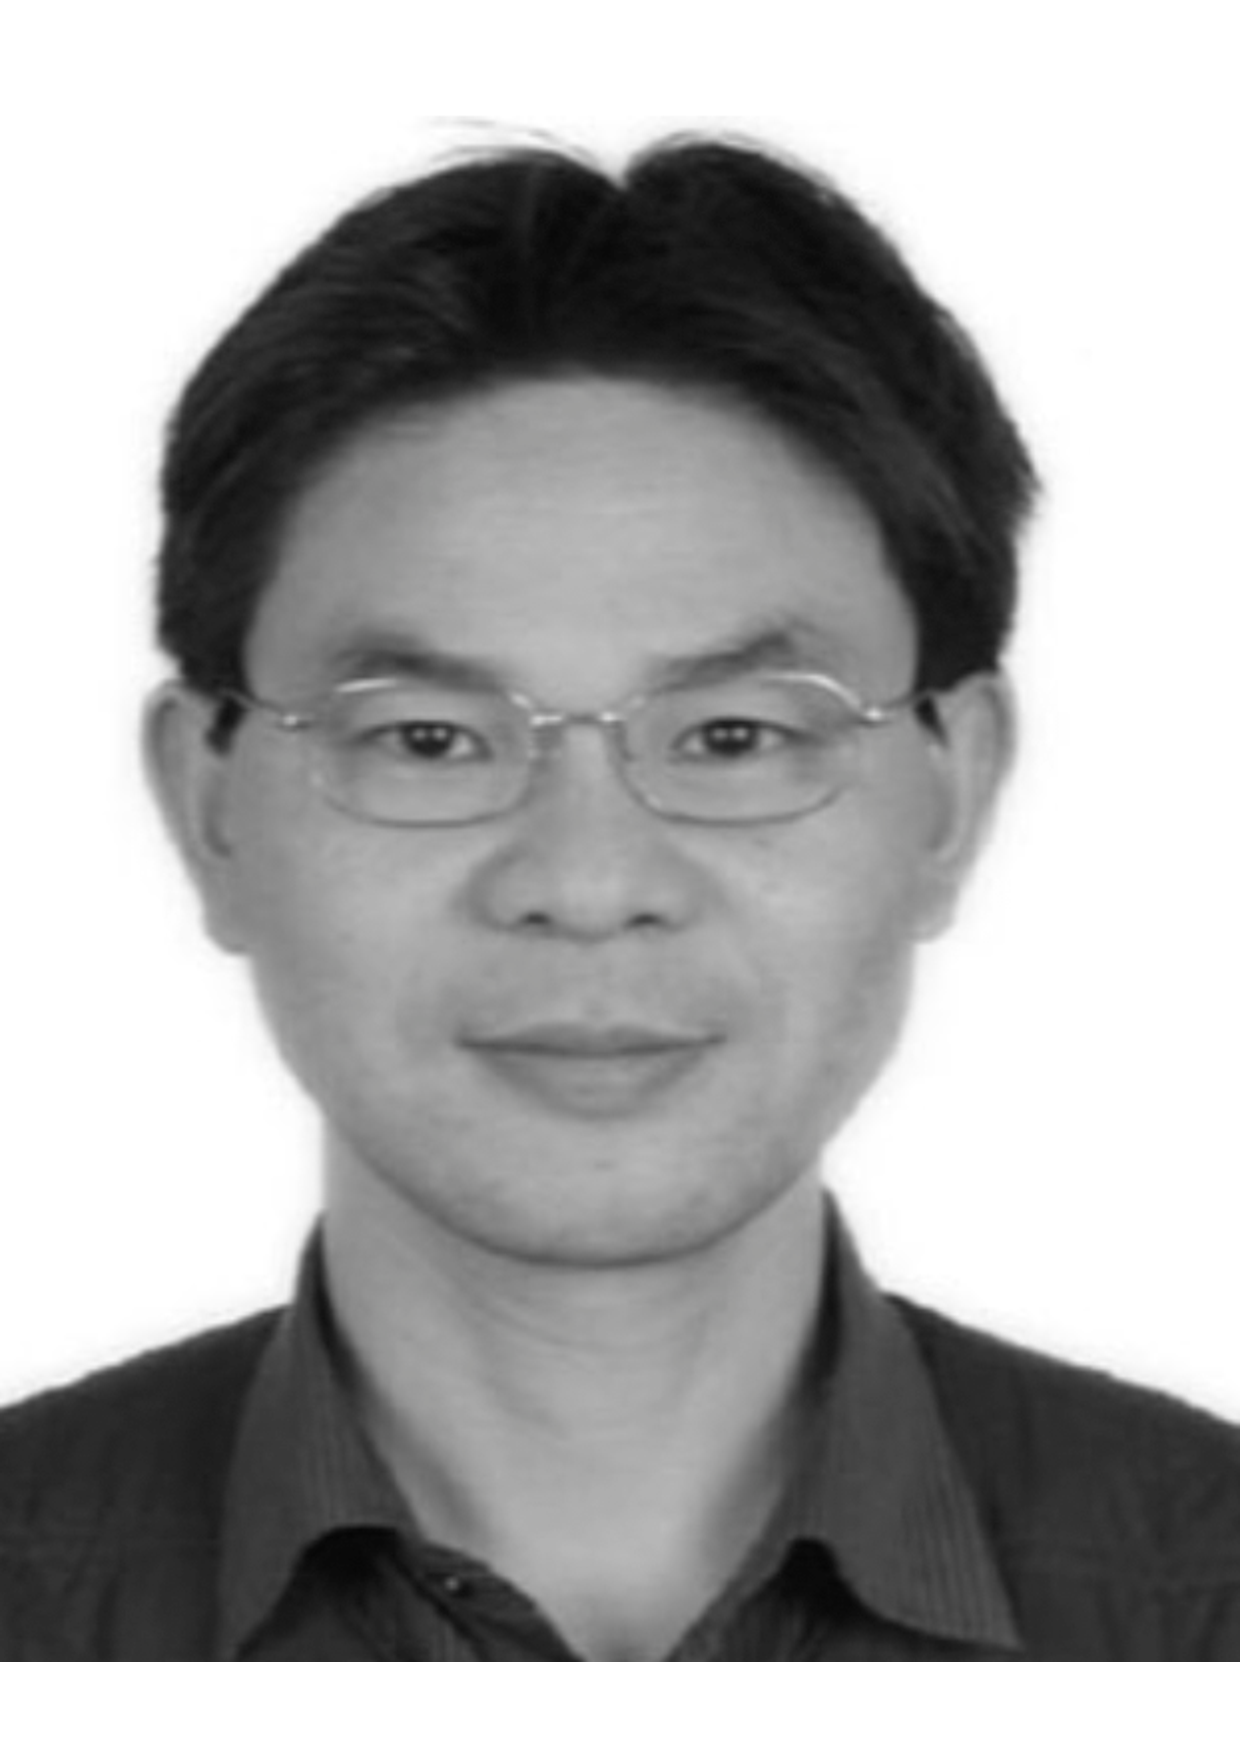
\includegraphics[width=1in,height=1.25in,clip,keepaspectratio]{./figs/cg.pdf}}]
{Guang Cheng} (Member,~IEEE) received the B.S. degree in traffic engineering from Southeast University, Nanjing, China, in 1994, the M.S. degree in computer application from the Hefei University of Technology, Hefei, China, in 2000, and the Ph.D. degree in computer network from Southeast University, in 2003.
He is currently a Full Professor with the School of Cyber Science and Engineering, Southeast University. He has authored or coauthored seven monographs and more than 100
technical papers, including top journals and top conferences. 
His research interests include network security, network measurement, and traffic behavior analysis.
\end{IEEEbiography}

\begin{IEEEbiography}
[{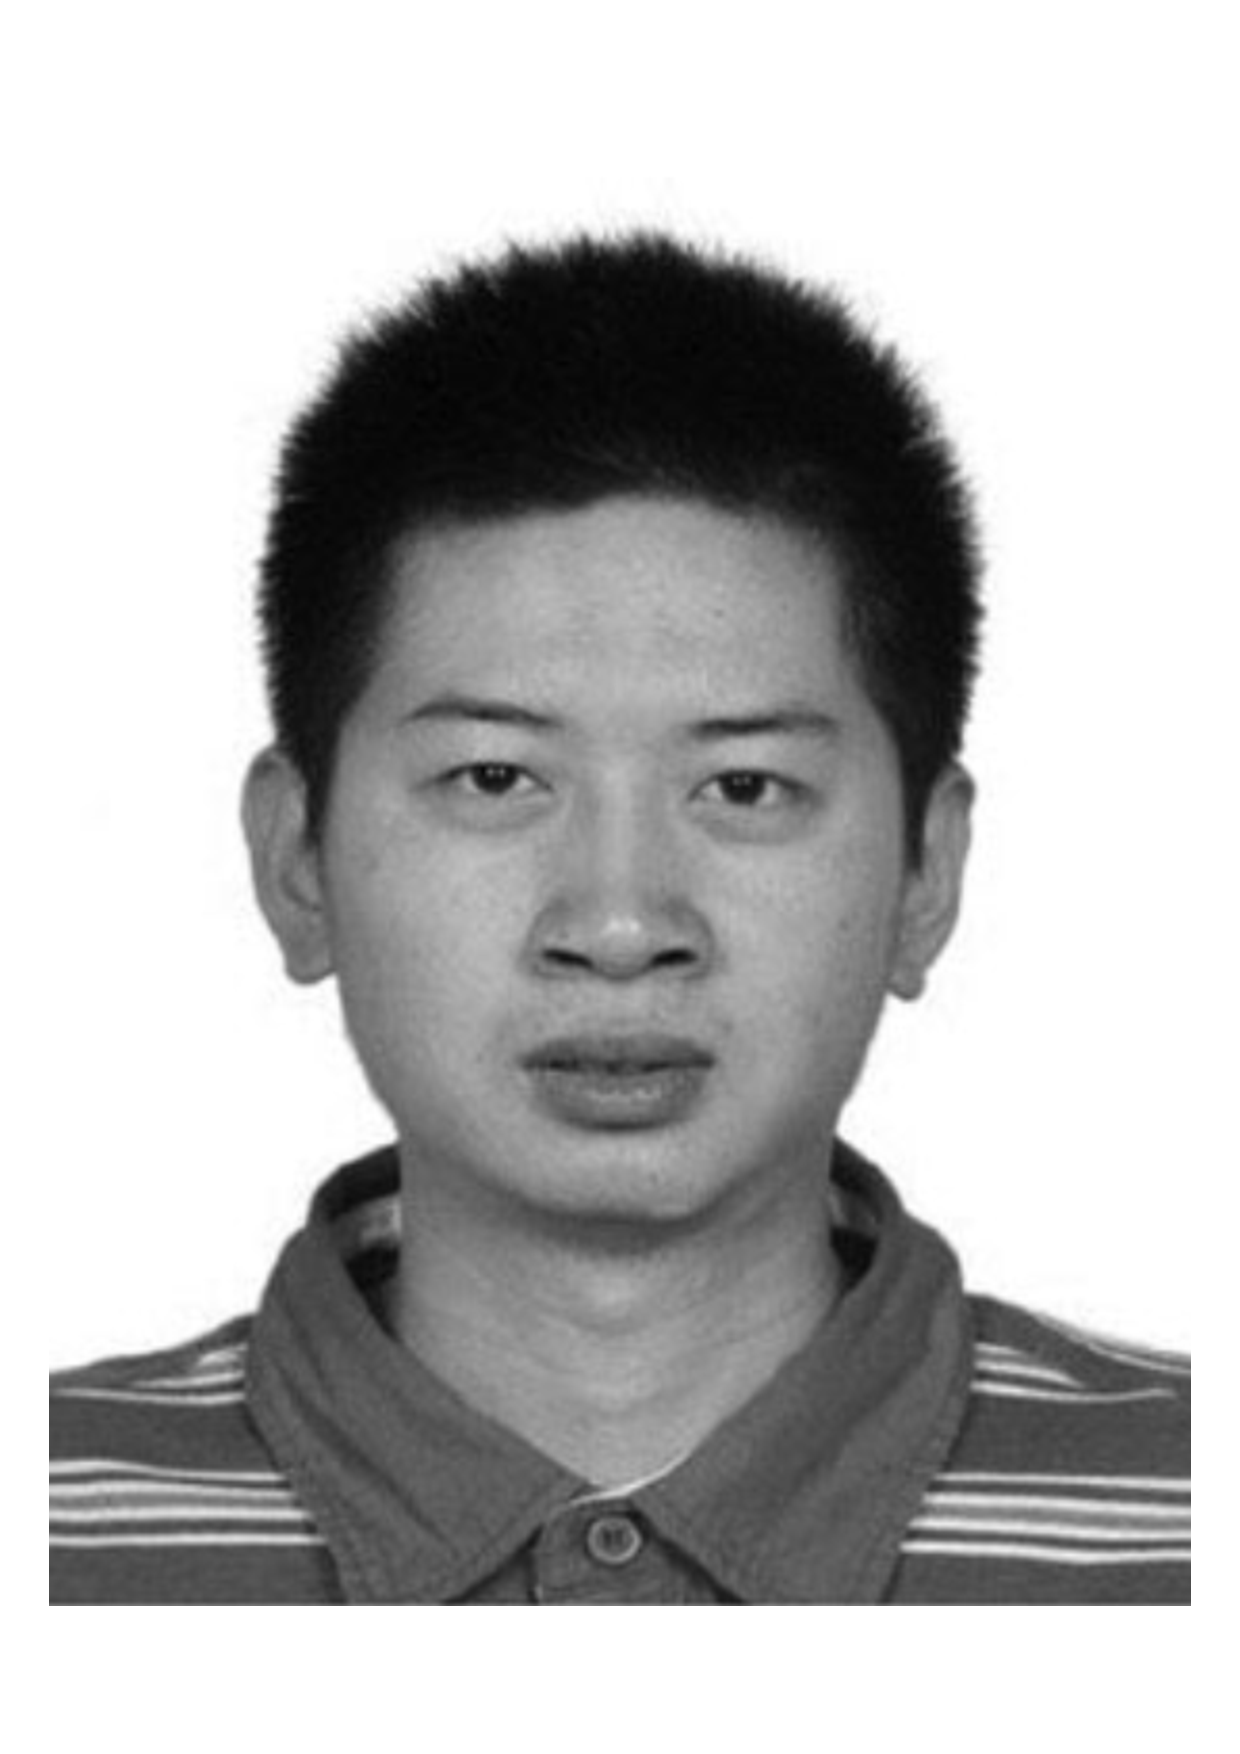
\includegraphics[width=1in,height=1.25in,clip,keepaspectratio]{./figs/zxj.pdf}}]
{Xinjie Zhao} received the B.S., M.S., and Ph.D. degrees from Ordnance Engineering College, Shijiazhuang, China, in 2006, 2009, and 2012, respectively.
He is currently with the College of Computer Science and Technology, Zhejiang University, Hangzhou, China. His main research interests include side channel analysis, fault analysis, and combined analysis in cryptography.
Dr. Zhao won the best paper award in COSADE 2012.
\end{IEEEbiography}

\begin{IEEEbiography}
[{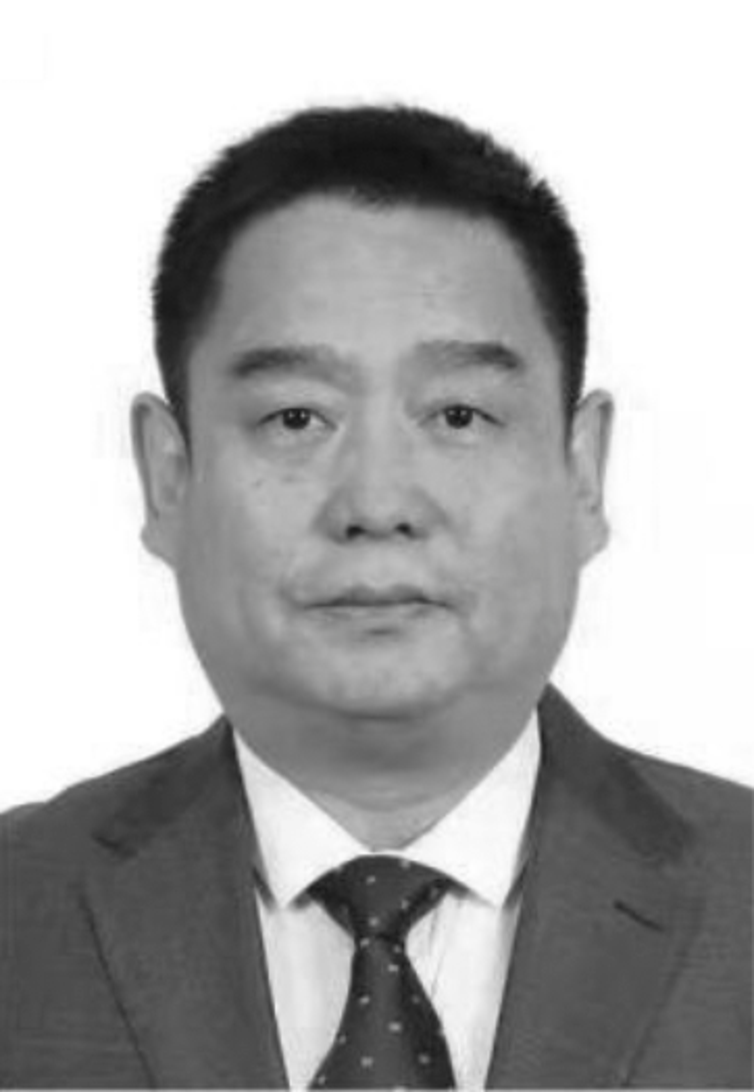
\includegraphics[width=1in,height=1.25in,clip,keepaspectratio]{./figs/gsz.pdf}}]
{Shize Guo} received the B.S. and M.S. degrees from Ordnance Engineering College, China, in 1988 and 1991, respectively, and the Ph.D. degree from the Harbin Institute of Technology, in 1994. He is currently with the College of Computer Science and Technology, Zhejiang University, Hangzhou, China. His main research interests include information technology and information security.
\end{IEEEbiography}

\vfill